% SPDX-FileCopyrightText: 2025 Jorge Teixeira Crespo <jorge.teixeira@udc.es>
%
% SPDX-License-Identifier: GPL-2.0-or-later

\chapter{Technology Selection}
\label{chap:technology-selection}

\lettrine{B}{ased} on the comparative analysis in the previous chapter, this section outlines the final decisions taken for each service in the infrastructure.  
Each subsection details the chosen solution, the motivation behind the decision, and the key trade-offs considered.  
As stated previously, the focus is on ensuring coherence with GPUL's values, long-term maintainability, and the practical constraints of a volunteer-run environment.

%--------------------------------------------------------------------
\section{Mailing-list Managers}

To modernize the mailing list service while ensuring archival continuity, the project will adopt Mailman 3, alongside the HyperKitty web archiver. The primary driver for this decision is ensuring continuity with the existing Mailman 2 deployment while significantly modernizing the service. Migrating to a different platform, such as Sympa, would jeopardize the integrity and accessibility of the historical archives, which are a critical resource for the association. In contrast, Mailman 3 offers a direct and well-documented upgrade path. The migration process is highly automated, with official tools like \texttt{mailman import21} for list configuration and \texttt{hyperkitty\_import} for archives, minimizing the risk of data loss and reducing the manual effort required~\cite{mailman-migration-docs}.

Beyond the seamless migration, Mailman 3's redesigned architecture presents a significant leap forward in terms of maintainability and features. The system is now modular, with a central \texttt{Mailman Core} handling message processing and a REST API for administration. This separation of concerns not only simplifies maintenance but also allows for flexible integration with other services. For users, the most visible improvement comes from HyperKitty, which replaces the outdated Pipermail archiver~\cite{hyperkitty-docs}. It provides a modern, searchable web interface where members can easily browse, search, and even reply to conversations directly, greatly improving the accessibility of the archives.

For list administration, the suite includes Postorius, a web-based front-end to the REST API~\cite{postorius-docs}. While optional—as all tasks can be performed via the command line—its user-friendly interface for managing lists and subscribers is a key advantage for a volunteer-run infrastructure. The platform's maturity and adoption by other large open-source projects, such as the Fedora Project, further reinforces this choice. Finally, the entire Mailman 3 suite is licensed under the GNU General Public License (GPL), which fully aligns with GPUL's commitment to using and promoting free and open-source software.

%--------------------------------------------------------------------
\section{Cloud Storage / Groupware}

For cloud storage and groupware, the project will continue to use the Nextcloud platform, upgrading the current deployment to Nextcloud Hub 10. The primary motivation for this decision is to ensure service continuity and leverage existing user familiarity. By staying within the Nextcloud ecosystem, members will not need to learn a new tool, which minimizes disruption and training overhead. The migration path is considered low-risk; a new, clean instance of Nextcloud Hub 10 will be deployed, and user data will be migrated by transferring the files directly and recreating the user accounts to ensure data integrity~\cite{nextcloud-docs}.

Furthermore, Nextcloud's status as a community-driven project licensed under the AGPL aligns with GPUL's core values, setting it apart from alternatives with a heavier enterprise focus. A key strategic advantage of this choice is the seamless integration with Nextcloud Talk, the selected video conferencing platform. This creates a unified groupware suite, providing a single, cohesive environment for file management, real-time communication, and collaboration, which simplifies the overall infrastructure and user workflow.

%--------------------------------------------------------------------
\section{Video Conferencing Platforms}

As anticipated in the previous section, video conferencing capabilities will be provided by Nextcloud Talk. This decision is primarily driven by its seamless integration into the Nextcloud Hub ecosystem, creating a single, unified platform for all of GPUL's collaborative needs. By leveraging the existing infrastructure, users can schedule meetings directly from the calendar, share documents from their cloud storage during a call, and manage conversations within the same familiar interface~\cite{nextcloud-talk-docs}.

While alternatives like Jitsi Meet or BigBlueButton offer more extensive features, they were deemed overly complex and resource-intensive for the association's requirements. GPUL's typical use case involves small-scale meetings with fewer than ten participants, for which Nextcloud Talk's capabilities are perfectly sufficient. Opting for a more heavyweight solution like BigBlueButton would impose an unnecessary strain on server resources without providing tangible benefits for day-to-day operations. Therefore, Nextcloud Talk represents the most pragmatic and efficient choice, providing robust functionality where it matters most—within a tightly integrated and resource-friendly groupware environment.

%--------------------------------------------------------------------
\section{Git Forges}

For code hosting and version control, all of GPUL's repositories will be consolidated on GitHub, leading to the decommissioning of the legacy \texttt{git daemon}. While this represents a move towards a proprietary, cloud-based service, it is a pragmatic decision driven by several factors. It provides continuity, as the platform is already in use for the association's most active projects, and it ensures operational resilience. Hosting the association's infrastructure-as-code and deployment scripts on an external, highly-available platform mitigates the critical risk of a circular dependency. If the self-hosted infrastructure were to fail, the code required to restore it would remain accessible, a crucial factor for a small, volunteer-run team.

Furthermore, GitHub is the de facto standard for open-source collaboration, meaning most potential contributors are already familiar with its workflows, lowering the barrier to entry. The platform also provides significant value through its integrated features. GitHub Actions offers a powerful CI/CD system for automating builds and deployments, while GitHub Pages allows for the effortless hosting of static websites, which is ideal for things like event landing pages~\cite{github-docs}. This strategic choice allows the team to focus its limited resources on other critical services rather than on maintaining a self-hosted forge.

%--------------------------------------------------------------------
\section{Team Chat Platforms}

To establish a sovereign, community-wide communication channel, the project will deploy a self-hosted Matrix homeserver using the Synapse implementation. The primary goal is to create a centralized communication platform for the entire GPUL community, moving away from the current reliance on proprietary services. While Nextcloud Talk can be used for focused, internal collaboration among the board and activity organizers, Matrix will serve as the open forum for all members, fostering the same vibrant, community-wide interaction that currently exists on platforms like Telegram.

Matrix's architecture is ideally suited for this role. Its support for distinct channels (rooms) with varying access levels allows for the creation of public spaces for general discussion alongside private groups for specific projects. A key feature influencing this decision is Matrix's native support for bridging, which will allow the existing, active Telegram group to be connected directly to the new server~\cite{matrix-docs}. This capability ensures a smooth and gradual transition for current members. A further advantage over platforms like Mattermost is that Matrix is an open standard, not a single product. This empowers users to select their preferred client from a diverse ecosystem, rather than being restricted to an official application. By adopting Matrix, GPUL is not only gaining a powerful communication tool but also championing a leading example of a federated, open-source standard, which aligns perfectly with the association's core mission.

%--------------------------------------------------------------------
\section{Secrets / Password Vault}

To replace the insecure plaintext password file, the project will implement Passbolt, a team-oriented password manager that aligns with GPUL's security and collaboration requirements. The decision was made after ruling out other alternatives for specific reasons. HashiCorp Vault, while powerful, was dismissed as an overly complex, enterprise-focused solution; its features, such as dynamic secret rotation, are overkill for the association's needs, and its Business Source License (BSL) does not align with the project's commitment to fully open-source software~\cite{vault-bsl}.

The primary decision came down to a comparison between Passbolt and Bitwarden. While both are excellent open-source options, they are designed with different use cases in mind. Bitwarden is primarily geared towards individual use, whereas Passbolt is built from the ground up for secure team collaboration. This is most evident in its sharing model: Passbolt allows for highly granular access control, enabling the sharing of individual passwords or specific folders with different users and teams, all while providing detailed audit logs of who accessed what, and when. This is a critical feature for managing shared credentials in a volunteer organization.

From a security standpoint, Passbolt's architecture provides a stronger model for team use. It relies on end-to-end GPG encryption, where each user has a unique private key for decryption~\cite{passbolt-security}. In contrast, systems like Bitwarden derive the encryption key from a user's master password. In a team environment, this means the effective security of a shared secret is only as strong as the weakest master password among the users it is shared with. Passbolt's model avoids this issue, ensuring a more robust and consistent security posture. For these reasons, Passbolt is the clear choice to replace the insecure plaintext password file.

%--------------------------------------------------------------------
\section{Monitoring \& Logging}

To establish comprehensive observability, the infrastructure will adopt the Prometheus, Grafana, and Loki combination, commonly known as the PLG stack. This decision prioritizes a balance of power, resource efficiency, and ease of use. While powerful, alternative stacks like ELK or OpenSearch were discarded due to their significant resource consumption and steeper learning curve, which were deemed inappropriate for a volunteer-managed infrastructure.

The final decision came down to a choice between the PLG stack and Zabbix. Both platforms are highly capable and would meet the association's technical requirements. However, the PLG stack holds a significant advantage in terms of community adoption and ecosystem vibrancy. While metrics like GitHub stars can be superficial (see Figure~\ref{fig:monitoring-stars}), the broader community sentiment and contributor data suggest that Grafana Labs fosters a significantly more community-centric development model. Projects like Grafana and Loki not only accept but actively encourage external contributions, with open governance models and a track record of fast response to community pull requests~\cite{collab-grafana}. In contrast, Zabbix development remains tightly controlled by the company, with limited avenues for non-employees to influence or contribute to the core platform~\cite{zabbix-dev-policy}.

\begin{figure}[H]
  \centering
  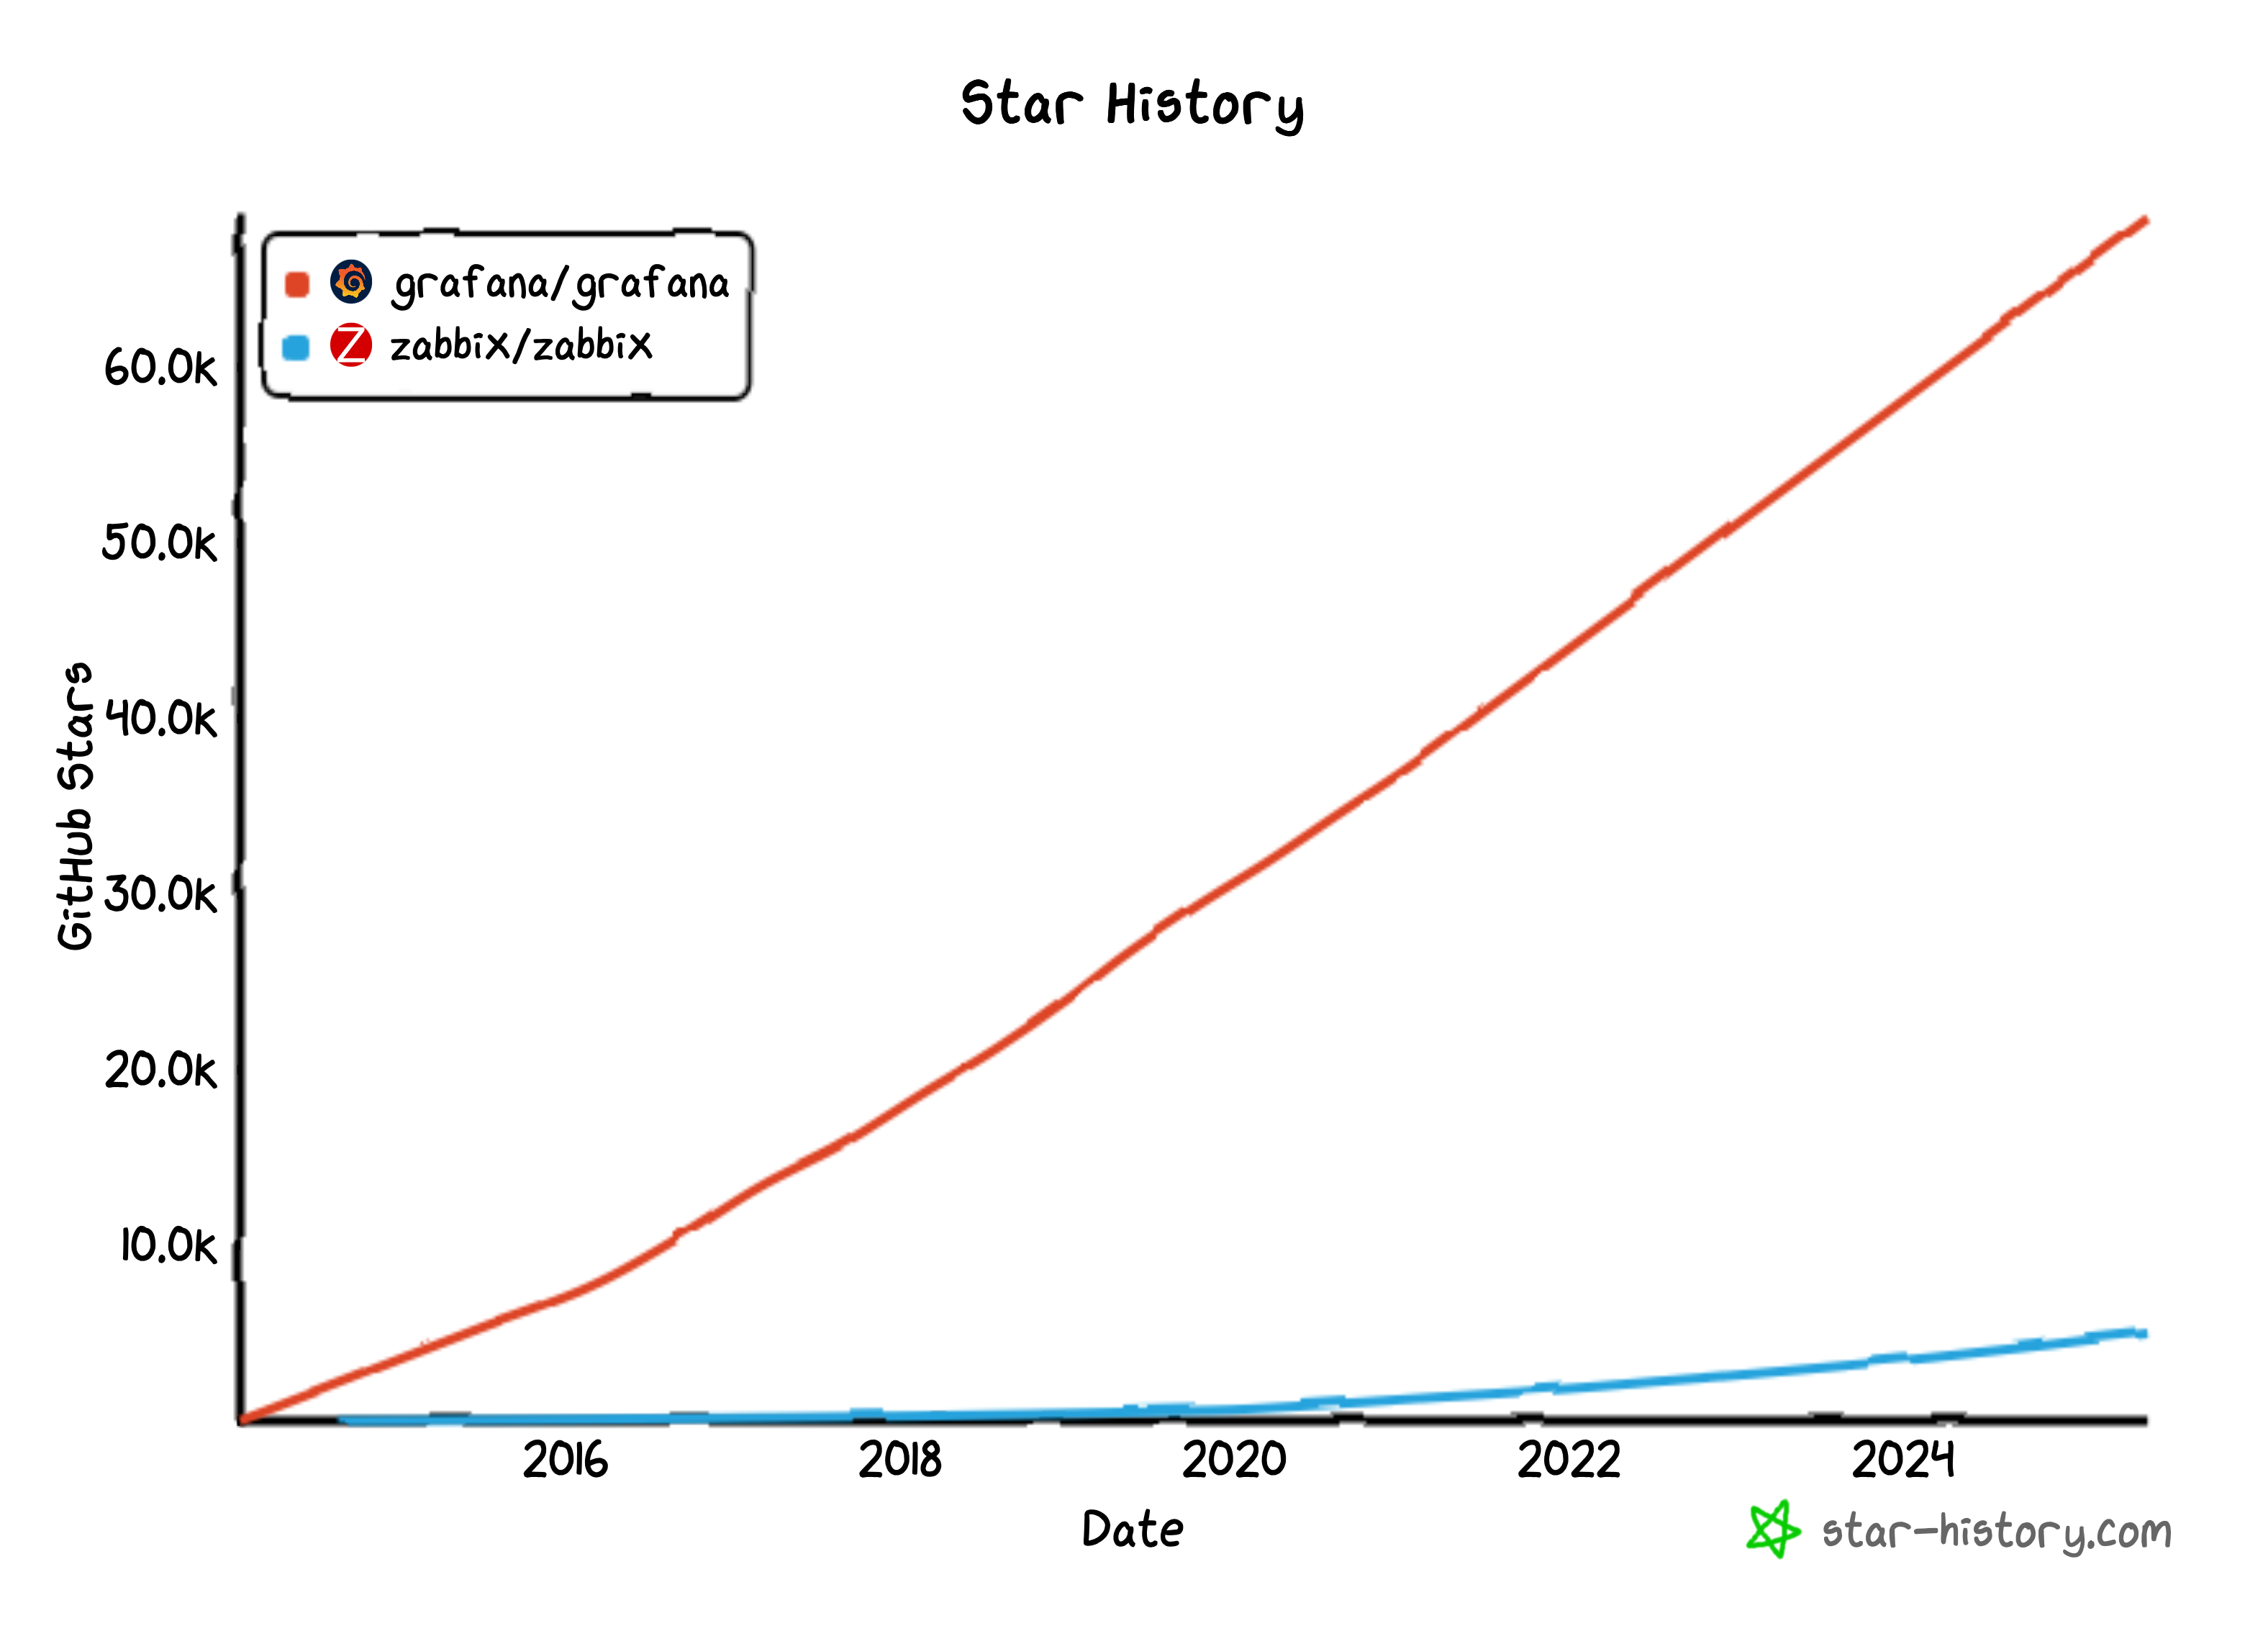
\includegraphics[width=0.9\textwidth]{imaxes/monitoring-stars.png}
  \caption{A historical comparison of GitHub stars for the Grafana and Zabbix projects. Source: \url{https://www.star-history.com}}
  \label{fig:monitoring-stars}
\end{figure}

Furthermore, the user experience and setup process heavily influenced the decision. The PLG stack is widely regarded as having a more intuitive setup and a more modern, user-friendly interface. Grafana, in particular, is renowned for its powerful and flexible visualization capabilities, making it easier to build meaningful dashboards. This view is supported by multiple online comparisons, which often highlight Grafana's superior ease of use for teams getting started with monitoring~\cite{squadcast-zabbix-grafana}. Combined with a large and responsive community, this gentle learning curve makes the PLG stack the most strategic choice for ensuring long-term maintainability in the context of a community-led infrastructure.

%--------------------------------------------------------------------
\section{Event Ticketing \& CFP Tooling}

Event management will be addressed via a phased migration, with the immediate step being the deployment of a self-hosted \textbf{pretalx} instance. This initial move is primarily driven by cost-efficiency, as it allows GPUL to stop paying for the hosted pretalx.com service while retaining the powerful call-for-proposals (CFP) and scheduling functionalities that the association already uses and values~\cite{pretalx-docs}.

For the time being, both Meetup and Eventbrite will remain in use for community outreach and paid ticketing, respectively. A full migration to a self-hosted stack is deferred due to significant non-technical considerations. Moving away from Meetup requires a careful community management strategy to avoid losing existing members and to mitigate the well-documented risk of abandoned groups being taken over by spammers, which would damage the association's reputation~\cite{combuilders-meetup-takeover}.

Similarly, replacing Eventbrite with a self-hosted alternative like pretix would necessitate integrating a third-party payment provider such as Stripe or PayPal. This carries administrative and financial responsibilities that require a formal decision from the board and is therefore considered future work. The current approach allows for an immediate cost saving while providing the time needed to address the broader strategic questions of community and financial management.

%--------------------------------------------------------------------
\section{Invoicing / Accounting}

To handle all invoicing and accounting needs, the project will implement FacturaScripts. This decision is primarily driven by the need for a solution that is both compliant with Spanish regulations and accessible to a rotating team of student volunteers. While Odoo is an extremely powerful ERP, its extensive feature set and significant learning curve were considered a disadvantage. The complexity would create a high barrier to entry for new treasurers, risking operational continuity.

FacturaScripts, in contrast, offers the ideal balance of functionality and simplicity for GPUL. As an open-source project developed in Spain, it is purpose-built to handle national fiscal requirements, including native support for Facturae and planned compliance with the upcoming VeriFactu system~\cite{FacturaScriptsAntifraude}. Its user interface is straightforward and focused on core accounting tasks, which dramatically simplifies the onboarding process for new volunteers. By providing all the necessary features without unnecessary complexity, FacturaScripts is the most sustainable choice for managing the association's finances long-term.

It is important to note that while the technical deployment of FacturaScripts will be completed as part of this project, the formal adoption for official accounting is an administrative decision reserved for the board. The final migration of financial data and processes will be carefully timed to coincide with a logical cutoff point, such as the end of a financial quarter or the start of a new fiscal year, to ensure a clean and orderly transition.

%--------------------------------------------------------------------
\section{Phone / VoIP Integration}

The university's analog phone line will be integrated into a modern VoIP system by deploying a self-hosted Asterisk server, managed via the FreePBX web interface. This combination represents the de facto standard for open-source telephony and is the only fully free and open-source alternative that meets the project's requirements~\cite{AsteriskFeatures}. Proprietary platforms like 3CX, while user-friendly, were not considered due to their licensing and cost structures.

The physical integration will be achieved using a Grandstream HT813 FXO gateway located in the GPUL office. This device will connect the analog line from the university's phone system to the Asterisk server, converting incoming and outgoing calls to SIP. To provide remote access for board members, the primary method will be deploying Grandstream HT801 Analog Telephone Adapters (ATAs) in their homes. This approach allows them to connect standard analog phones to the VoIP system, offering a reliable, physical device for making and receiving calls.

This hardware-based strategy is explicitly preferred over relying on softphone applications for mobile devices. Softphones often experience reliability issues on modern operating systems due to aggressive background process management and limited ongoing development, rendering them unsuitable for critical communications. By using dedicated ATAs, the solution ensures dependable remote access to the association's phone line for key personnel.

%--------------------------------------------------------------------
\section{Service Deployment and Management}

The underlying foundation for service deployment and management will be Incus. This decision is the result of a careful evaluation of the project's core requirements: long-term maintainability, operational simplicity for a volunteer team, and the ability to cleanly isolate services without excessive overhead. The most complex alternatives were discarded early on; Kubernetes, while powerful, is designed for multi-node orchestration and its complexity is unwarranted for a single-server deployment~\cite{KubernetesDocs2025}.

The primary contenders were Proxmox, Incus, and a bare Docker/Podman installation on a standard Linux distribution. A "bare Docker" approach was ruled out because many of the selected services are best maintained when installed directly on an operating system, following their official documentation. Forcing every service into a Docker container would often mean relying on unofficial, community-maintained images, which could complicate future maintenance. The goal is to keep each service's setup as close to the "vanilla" recommended installation as possible.

This leads to the core strategy of using system containers. Unlike application containers (like Docker), system containers (as managed by Incus) provide a full operating system userspace, sharing only the host's kernel~\cite{IncusLinuxContainers2023}. This allows each service to be installed in its own clean, isolated OS environment—for example, its own Debian container—while following the official installation guides as if it were on a dedicated machine. This approach also offers great flexibility: for services that are best deployed with Docker, a single system container can be set up with Docker installed inside it, providing a dedicated and isolated environment for running those specific application containers.

With the choice narrowed to platforms providing system containers, Incus emerged as the clear winner over Proxmox for this use case. Proxmox is an excellent, hypervisor-centric platform, but its primary advantages—a comprehensive web interface and robust virtual machine management—are not required here. The infrastructure will be managed via the command line by administrators comfortable with SSH, and there is no immediate need for full hardware virtualization. Incus provides exactly what is needed: a powerful, lightweight, and CLI-driven tool for managing system containers. As a thriving, community-led fork of LXD, it is the most efficient and versatile foundation for building a maintainable and reproducible infrastructure.
